\documentclass[12pt]{article}
\usepackage{graphicx}
\usepackage{subfigure}
\usepackage{epsfig}
\pagestyle{empty}

\begin{document}

\title{Problem E \\ All Rectangles}
\author{Input file: {\em pa.in} \\ Time limit: 3 seconds}
\date{}
\maketitle
\thispagestyle{empty}

\subsection*{Problem Description}

Geometrically, any rectangle has a unique, well-defined centre point. On a grid this is only true if the sides of the rectangle are an odd number of points long. We characterize any such rectangle by specifying an integer $k$. Define the left/right sides of a rectangle as width and top/bottom sides as length. We say that a rectangle with length/width equal to $4k+1/2k+1$ has size $k$. Now define a pattern of rectangles as follows.

\begin{enumerate}
  \item The largest rectangle is of size $k$ (i.e., length$/$width is $4k+1/2k+1$), which is centred in a $2048 \times 2048$ grid.
  \item The smallest permissible rectangle is of size 1 and the largest is of size 256, thus $1 \le k \le 256$.
  \item All rectangles of size $k > 1$ have a rectangle of size $k$ div 2 centred on each of their four corners. (Div implies integer division, thus 9 div 2 = 4).
  \item The top left corner of the grid has coordinates (0,0), the bottom right has coordinates (2048, 2048).
\end{enumerate}

Hence, given a value of $k$, we can draw a unique pattern of rectangles according to the above rules. Furthermore any point on the screen will be surrounded by zero or more rectangles. (If the point is on the border of a rectangle, it is considered to be surrounded by that rectangle). For example, if the size of the largest rectangle is given as 8, then the following rectangles would be produced.

        \begin{figure}[!h]
        \centering
        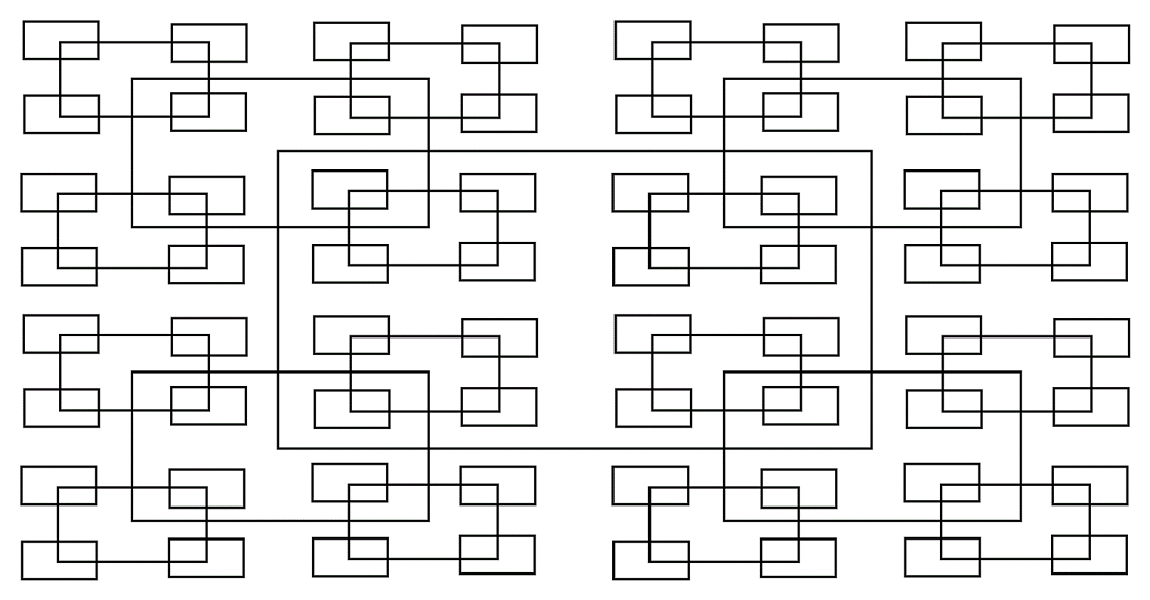
\includegraphics[scale=0.6]{Rectangle.eps}
        \label{fig:fig3.3}
        \end{figure}

Write a program that will read in a value of $k$ and the coordinates of a point, and will determine how many rectangles surround the point.


\subsection*{Input Format}

Input will consist of a series of lines. Each line will consist of a value of $k$ and the coordinates of a point, separated by a space. The file will be terminated by a line consisting of three zeroes (0 0 0).

\subsection*{Output Format}

Output will consist of a series of lines, one for each line of the input. Each line will consist of the number of rectangles containing the specified point.

\subsection*{Sample Input}
\begin{verbatim}
7 1014 1019
216 1000 1000
0 0 0
\end{verbatim}

\subsection*{Sample Output}
\begin{verbatim}
3
2
\end{verbatim}

\end{document}
